\documentclass[conference]{IEEEtran}
\usepackage[utf8]{inputenc}
\usepackage[T1]{fontenc}
\usepackage{amsmath,amssymb,amsfonts}
\usepackage{graphicx}
\usepackage{booktabs,tabularx}
% Permitir figuras antes de su texto en la misma página, sin cruzar el cierre.
\usepackage[above]{placeins}
\usepackage[authoryear,round]{natbib}
\usepackage{url}
\usepackage{hyperref}

% Una columna: colocación local flexible. Dos columnas: parte superior (!t).
% Sin barreras entre las subsecciones exploratorias: el texto puede llenar las columnas.
% Se conserva la barrera al cerrar la sección para no adelantar la siguiente.
% Permitir compilar desde docs/ o desde la raíz del proyecto.
\graphicspath{{../public/images/}{public/images/}}
\hypersetup{colorlinks=true,linkcolor=black,citecolor=black,urlcolor=blue}
\urlstyle{same}
\renewcommand{\IEEEkeywordsname}{Palabras clave}
\renewcommand{\bibsection}{\section*{Referencias}}
\renewcommand{\bibfont}{\footnotesize}
\setlength{\bibhang}{1.5em}
\setlength{\bibsep}{0.6\baselineskip}
\setlength{\emergencystretch}{1em}

\begin{document}

\title{Clasificación de modelos de carros mediante CNN's y propuestas de mejora}

\author{\IEEEauthorblockN{Yael Charles Marin}
\IEEEauthorblockA{\textit{A01711111} \\
\textit{Tecnológico de Monterrey Campus Querétaro}\\
Inteligencia artificial avanzada para la ciencia de datos \\
Grupo 601}}

\maketitle

\begin{abstract}
La clasificación de carros requiere reconocer diferencias entre modelos que pueden compartir formas, colores y escenarios. En este trabajo se analiza una red neuronal convolucional entrenada desde cero para distinguir diez modelos a partir del dataset Car Model Image Classification. Se parte de 2,084 imágenes y se estudian la distribución de clases, las dimensiones, la calidad visual, los duplicados y la procedencia. La limpieza retira 18 imágenes por conflictos de etiquetas, repetición exacta o similitud, las 2,066 restantes se transforman a RGB de $224\times224$ píxeles y se dividen de manera estratificada en entrenamiento, validación y prueba. La red contiene cuatro bloques convolucionales y 115,242 parámetros, y utiliza ReLU, max pooling, Adam y detención temprana. Con los mejores pesos de validación se obtiene una exactitud aproximada de 0.464 en entrenamiento, 0.294 en validación y 0.310 en prueba. El F1 macro de prueba es 0.273. Las curvas muestran sobreajuste y la matriz de confusión evidencia un desempeño desigual entre clases. Se discuten la concentración de autores, la ambigüedad de algunas imágenes y la posible pérdida de información por el preprocesamiento y la reducción espacial. Los resultados constituyen una referencia inicial y muestran que una arquitectura compacta necesita acompañarse de datos representativos y una evaluación cuidadosa de la generalización.
\end{abstract}

\begin{IEEEkeywords}
Clasificación de imágenes, carros, redes neuronales convolucionales, análisis exploratorio, sobreajuste, evaluación multiclase.
\end{IEEEkeywords}

\section{Introducción}

Identificar el modelo de un carro a partir de una imagen parece una tarea sencilla cuando se observan sus logos o su forma completa. Sin embargo, las fotografías pueden mostrar únicamente un faro, el interior o una vista parcial. También pueden contener varios vehículos, modificaciones estéticas y fondos que se repiten. Por esta razón, el problema no consiste solamente en identificar que hay un carro, sino en encontrar características que permitan distinguir una categoría de otra a pesar de esas variaciones.

Una red neuronal convolucional, o CNN, permite aprender patrones visuales mediante filtros que se ajustan durante el entrenamiento. En este proyecto se utiliza una CNN propia para clasificar diez modelos de carros. El interés está en analizar qué información recibe la red, qué se conserva o se pierde al preparar las imágenes y hasta qué punto el desempeño observado se mantiene en ejemplos que no actualizan los pesos.

Se toma como referencia el análisis exploratorio de imágenes de \citet{zhang2024}, que propone pasar del procesamiento y las mediciones a la identificación e interpretación de patrones. Este enfoque resulta útil para relacionar los hallazgos del dataset con decisiones concretas, sin considerar que toda diferencia observada representa automáticamente un defecto. El estudio de \citet{khan2026} aporta una discusión sobre desbalance y evaluación de clases minoritarias. Por su parte, Appasami y Savarimuthu (\citeyear{appasami2025}) estudian arquitecturas ligeras y el efecto de configurar convoluciones, pooling y entrenamiento.

En particular, \citet{khan2026} comparan modificaciones de la función de pérdida, muestreo y aumento de datos. Sus resultados muestran que incrementar ejemplos no garantiza una mejora equivalente de las clases minoritarias. Esto respalda analizar la recuperación por categoría antes de elegir una estrategia de balance.

Appasami y Savarimuthu (\citeyear{appasami2025}) estudian conjuntamente kernel, pooling y tamaño de lote. Su configuración destacada utiliza kernel $4\times4$, pooling $4\times4$ y lote de 64, además de mecanismos como dropout y aumento de datos.

\section{Fuente de datos y análisis exploratorio}

\subsection{Origen, tamaño y características}

Se utiliza el dataset \textit{Car Model Image Classification}, publicado en Kaggle por el usuario lightangle \citep{dataset}. Al momento de cargar los datos, se conserva una copia local de las imágenes y sus metadatos, lo que permite separar el material de origen de las transformaciones posteriores.

El dataset analizadp contiene 2,084 imágenes distribuidas en diez clases. Los metadatos incluyen clase, nombre del archivo, título, creador, licencia, versión de licencia, fuente y enlaces de procedencia. La fuente declarada es Flickr en 2,083 registros y Sketchfab en uno.

La Tabla~\ref{tab:distribucion} muestra todas las clases que contiene el dataset y la distribución de imágenes que pertenecen a cada clase.

\begin{table}[!htbp]
\caption{Distribución de los datos por clase}
\label{tab:distribucion}
\centering
\scriptsize
\setlength{\tabcolsep}{3pt}
\begin{tabular}{lr}
\toprule
Clase & Original \\
\midrule
Audi R8 & 231 \\
Audi RS5 & 124 \\
BMW M3 & 233 \\
BMW M5 & 239 \\
Chevrolet Camaro & 225  \\
Ford Mustang & 238 \\
Mercedes AMG GT & 147 \\
Nissan GT-R & 216 \\
Porsche 911 & 225 \\
Toyota Supra & 206 \\
\midrule
Total & 2,084 \\
\bottomrule
\end{tabular}
\par\smallskip
\end{table}

\subsection{Balance de clases y diversidad visual}

BMW M5 es la clase original más numerosa, con 239 imágenes, mientras que Audi RS5 tiene 124. En terminos de porcentaje son aproximadamente 11.47\% y 5.95\%, respectivamente, y la razón entre ambos conteos es 1.93. Hay un desbalance que debe tomarse en cuenta.

Una posbile consecuencia de este desbalanceo es que acertar en las clases más frecuentes puede elevar la exactitud global aun cuando otras categorías se reconozcan poco. Por ello, es importante considerar esto más adelante.

La Figura~\ref{fig:muestras} muestra cuatro ejemplos por clase, seleccionados de forma aleatoria. Se observan diferentes cambios en la perspectiva, iluminación y fondo. También aparecen interiores, acercamientos y escenas con varios vehículos. Estos ejemplos sugieren que el dataset incluye tanto variación visual válida como posibles problemas de relevancia o etiquetado.

\begin{figure}[!htbp]
\centering
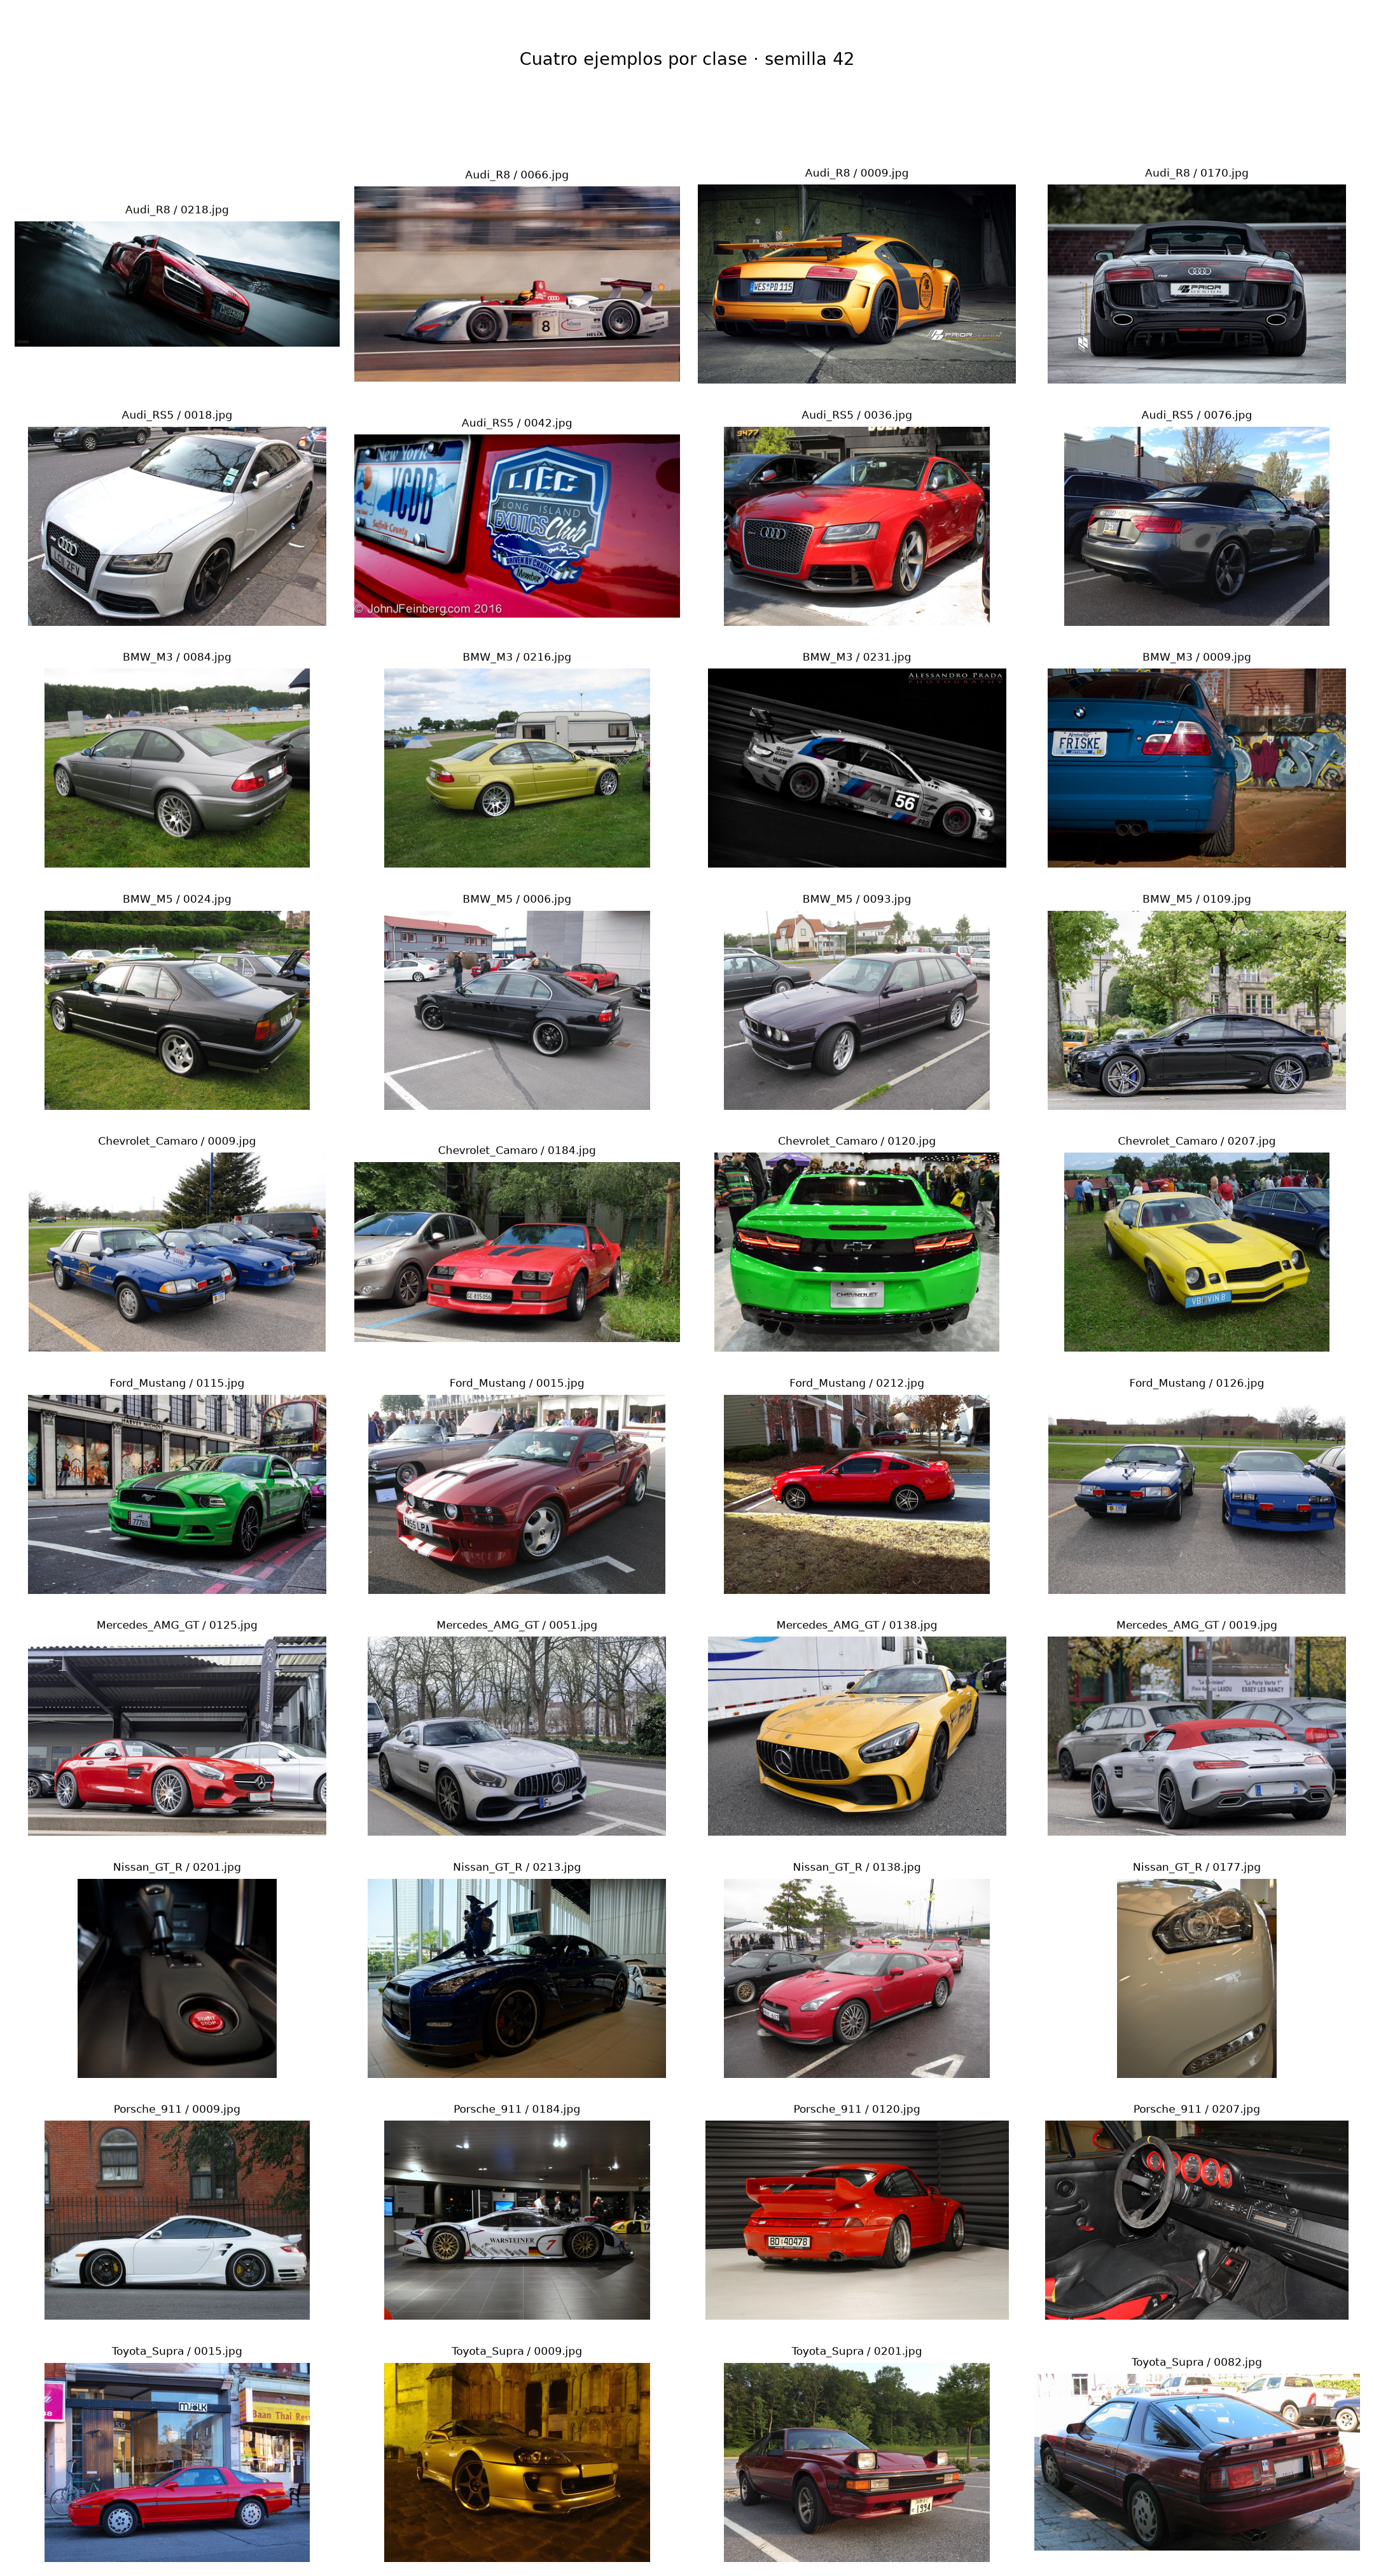
\includegraphics[width=\columnwidth,height=0.60\textheight,keepaspectratio]{eda/eda_muestras_clases.png}
\caption{Cuatro ejemplos originales por clase, con semilla 42.}
\label{fig:muestras}
\end{figure}

\subsection{Dimensiones, proporciones y calidad visual}

La Figura~\ref{fig:dimensiones} resume dimensiones, resolución, relación de aspecto y tamaño del archivo. El ancho mediano es de 1,024 píxeles y el alto mediano es de 685, estos valores representan medianas marginales y no implican que todas las imágenes tengan esa combinación, la resolución mediana es 0.701 megapíxeles, con valores entre 0.154 y 2.074, finalmente, la relación ancho/alto varía entre 0.562 y 3.373. Por lo tanto, forzar directamente todas las imágenes a un cuadrado modificaría sus proporciones.

\begin{figure}[!htbp]
\centering
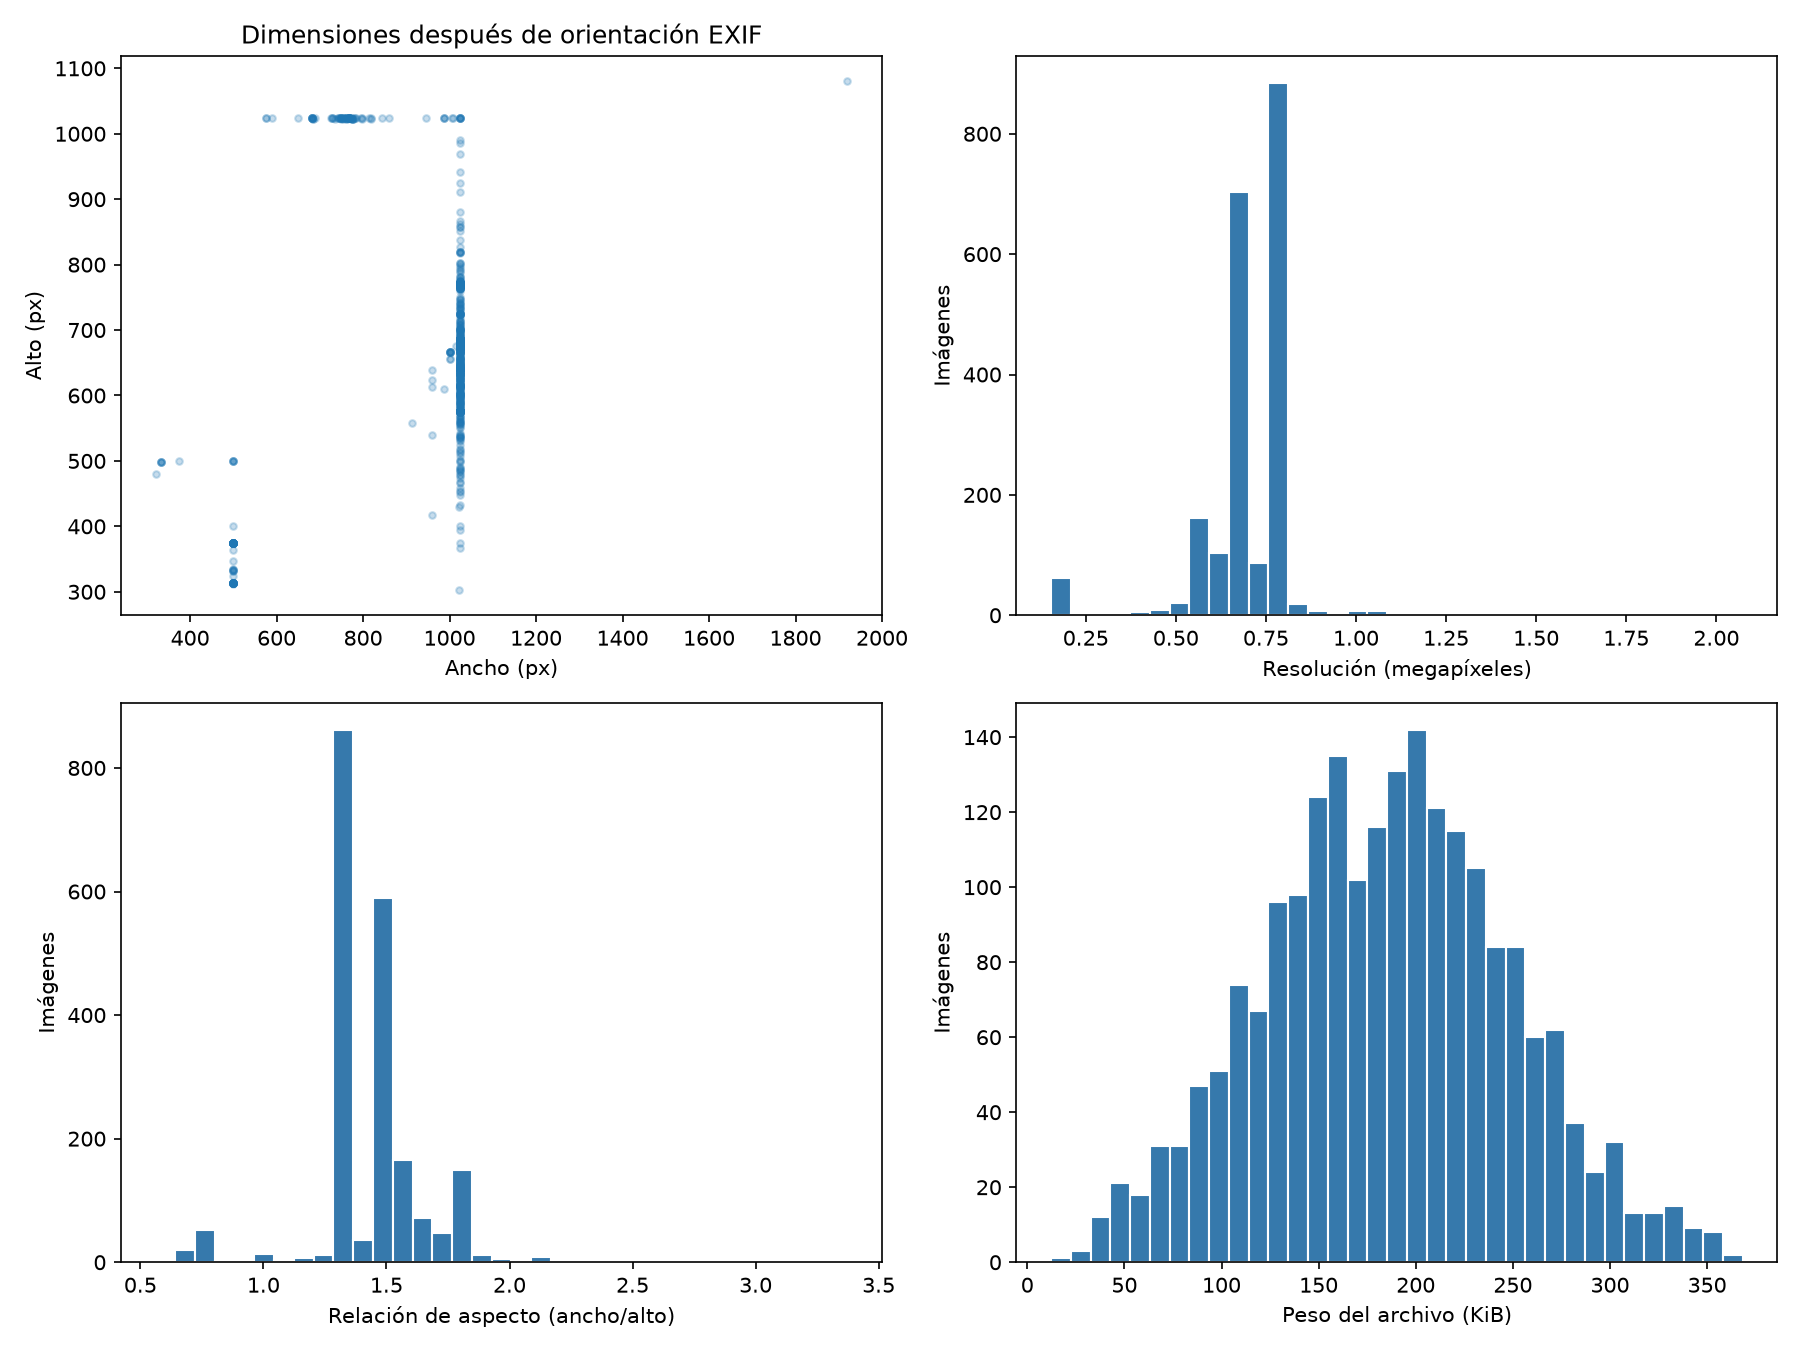
\includegraphics[width=\columnwidth]{eda/eda_dimensiones_peso.png}
\caption{Dimensiones corregidas por orientación EXIF, resolución, relación de aspecto y peso de las imágenes originales.}
\label{fig:dimensiones}
\end{figure}

El tamaño mediano de una imagen es 186.362 KiB, es importante distinguir que un archivo mayor no necesariamente aporta más información útil, además el modelo requiere una entrada uniforme que conserve la geometría de la carrocería.

En la Figura~\ref{fig:calidad} se observan distribuciones y valores extremos por clase.

\begin{figure*}[!t]
\centering
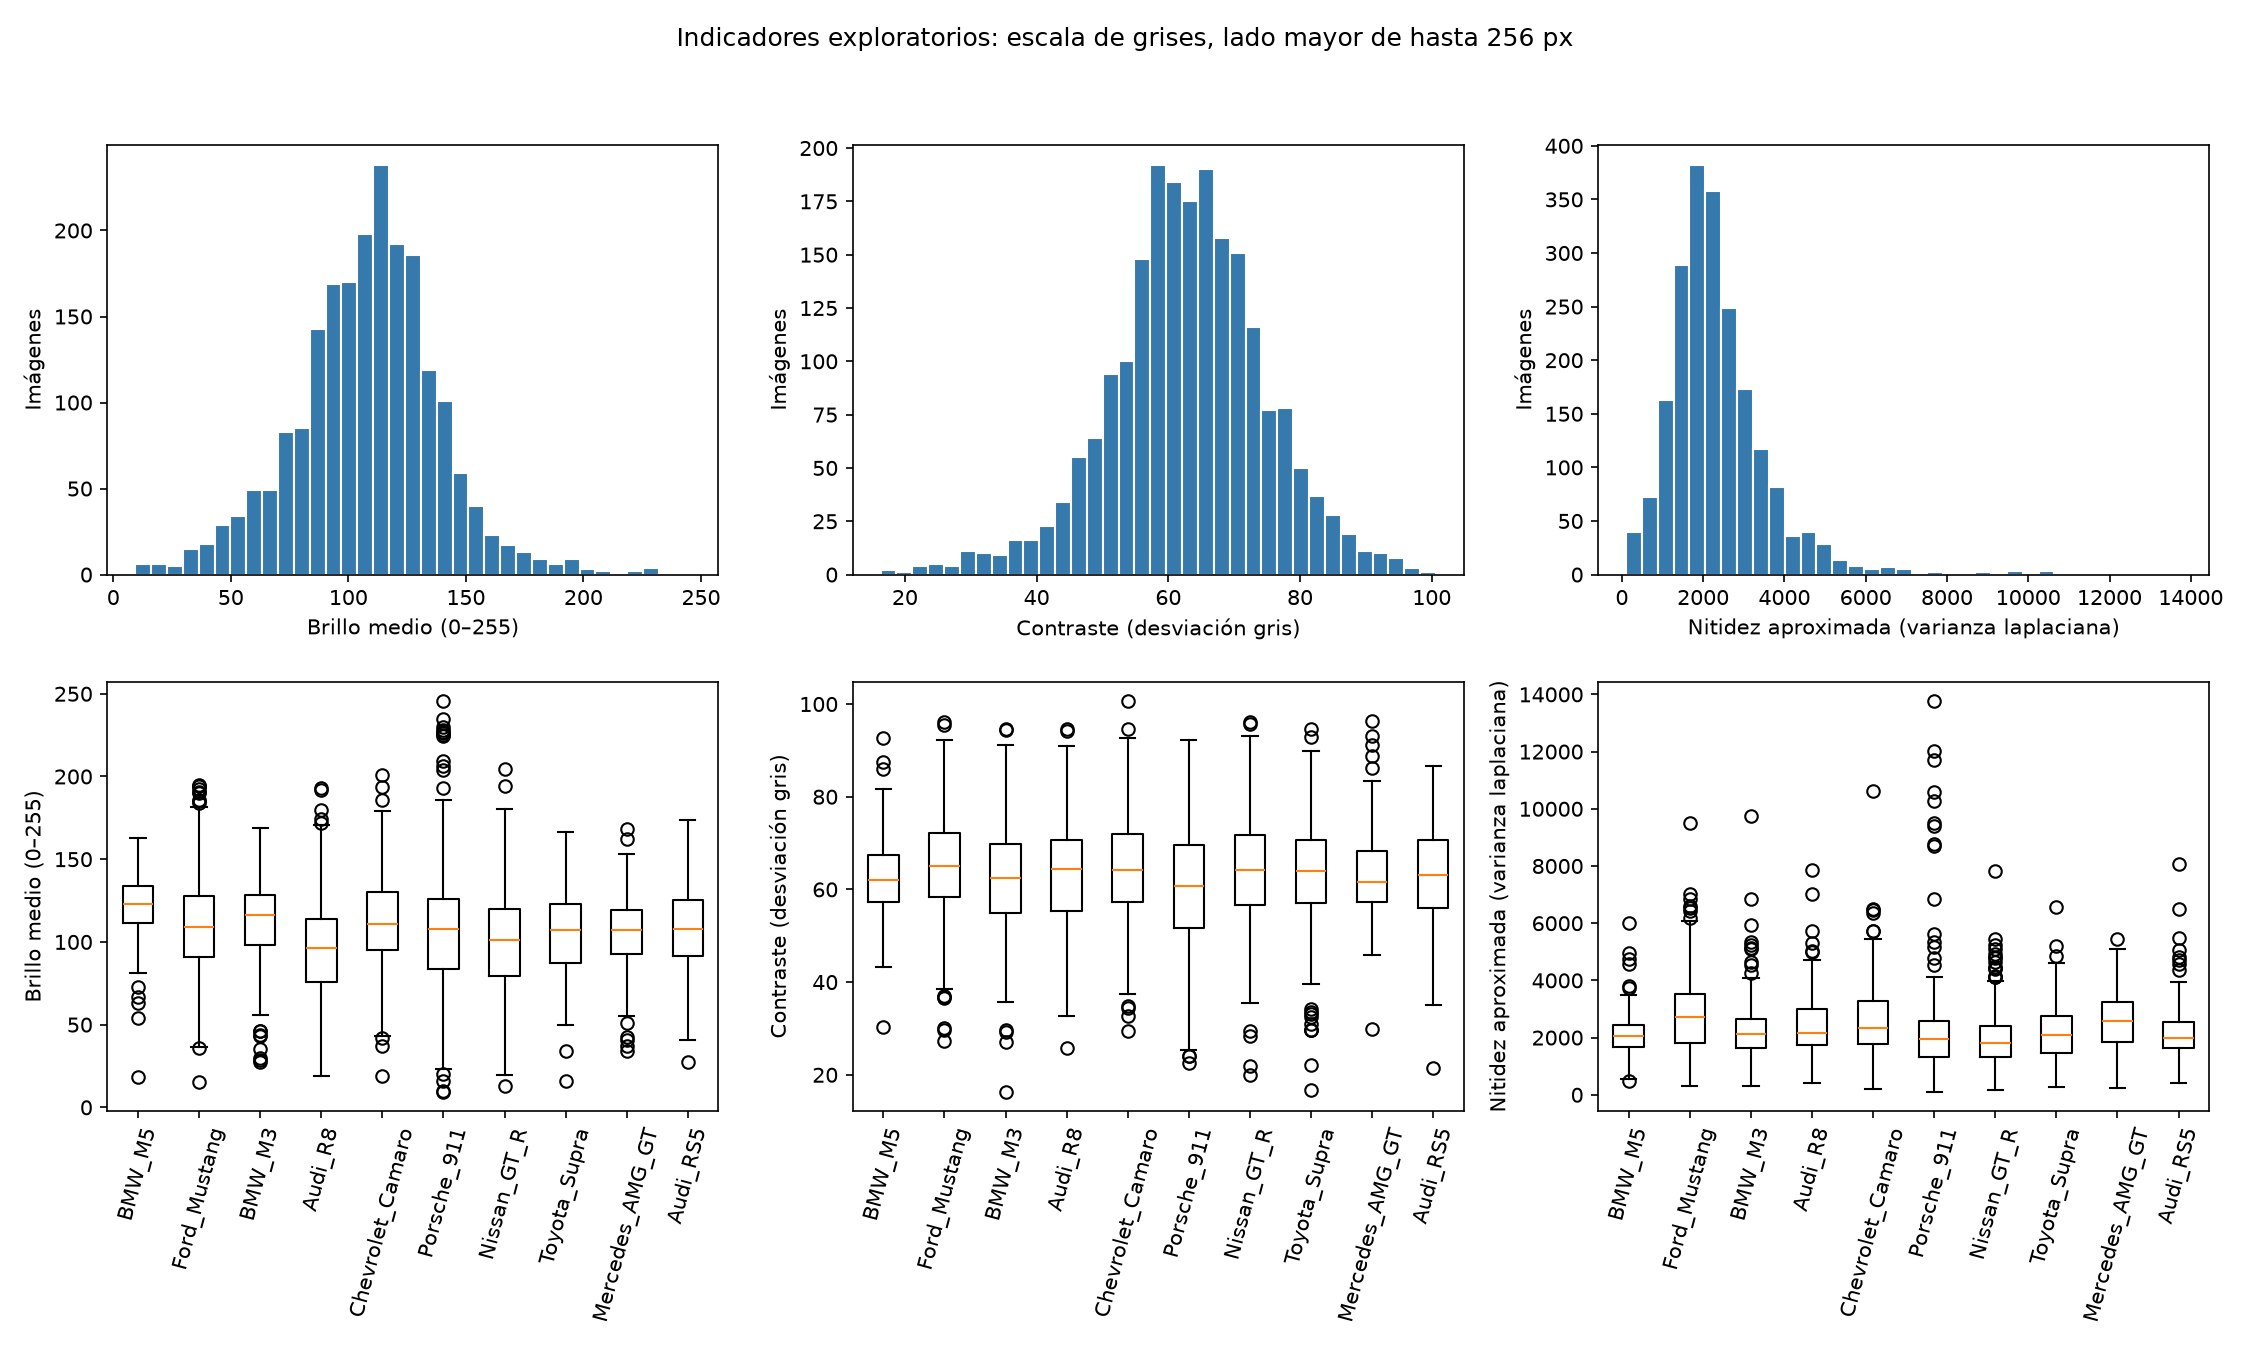
\includegraphics[width=0.92\textwidth,height=0.40\textheight,keepaspectratio]{eda/eda_calidad_visual.png}
\caption{Indicadores exploratorios de brillo, contraste y nitidez aproximada, globales y por clase.}
\label{fig:calidad}
\end{figure*}

La nitidez aproximada tiene una mediana de 2,150.608 y una cola hacia la derecha (valores altos), por ejemplo un fondo con muchos bordes puede aumentar este indicador sin que el carro se distinga mejor, un brillo extremo no justifica eliminar una imagen.

\subsection{Procedencia y concentración de autores}

En BMW M5, 218 de las 239 imágenes originales, equivalentes a 91.21\%, pertenecen al creador nakhon100. Ese mismo creador aporta 116 de las 233 imágenes de BMW M3, o 49.79\%. En Audi R8, Prior Design NA concentra 135 de 231 imágenes, aproximadamente 58.44\%. La Figura~\ref{fig:autores} muestra estas concentraciones.

\begin{figure*}[!t]
\centering
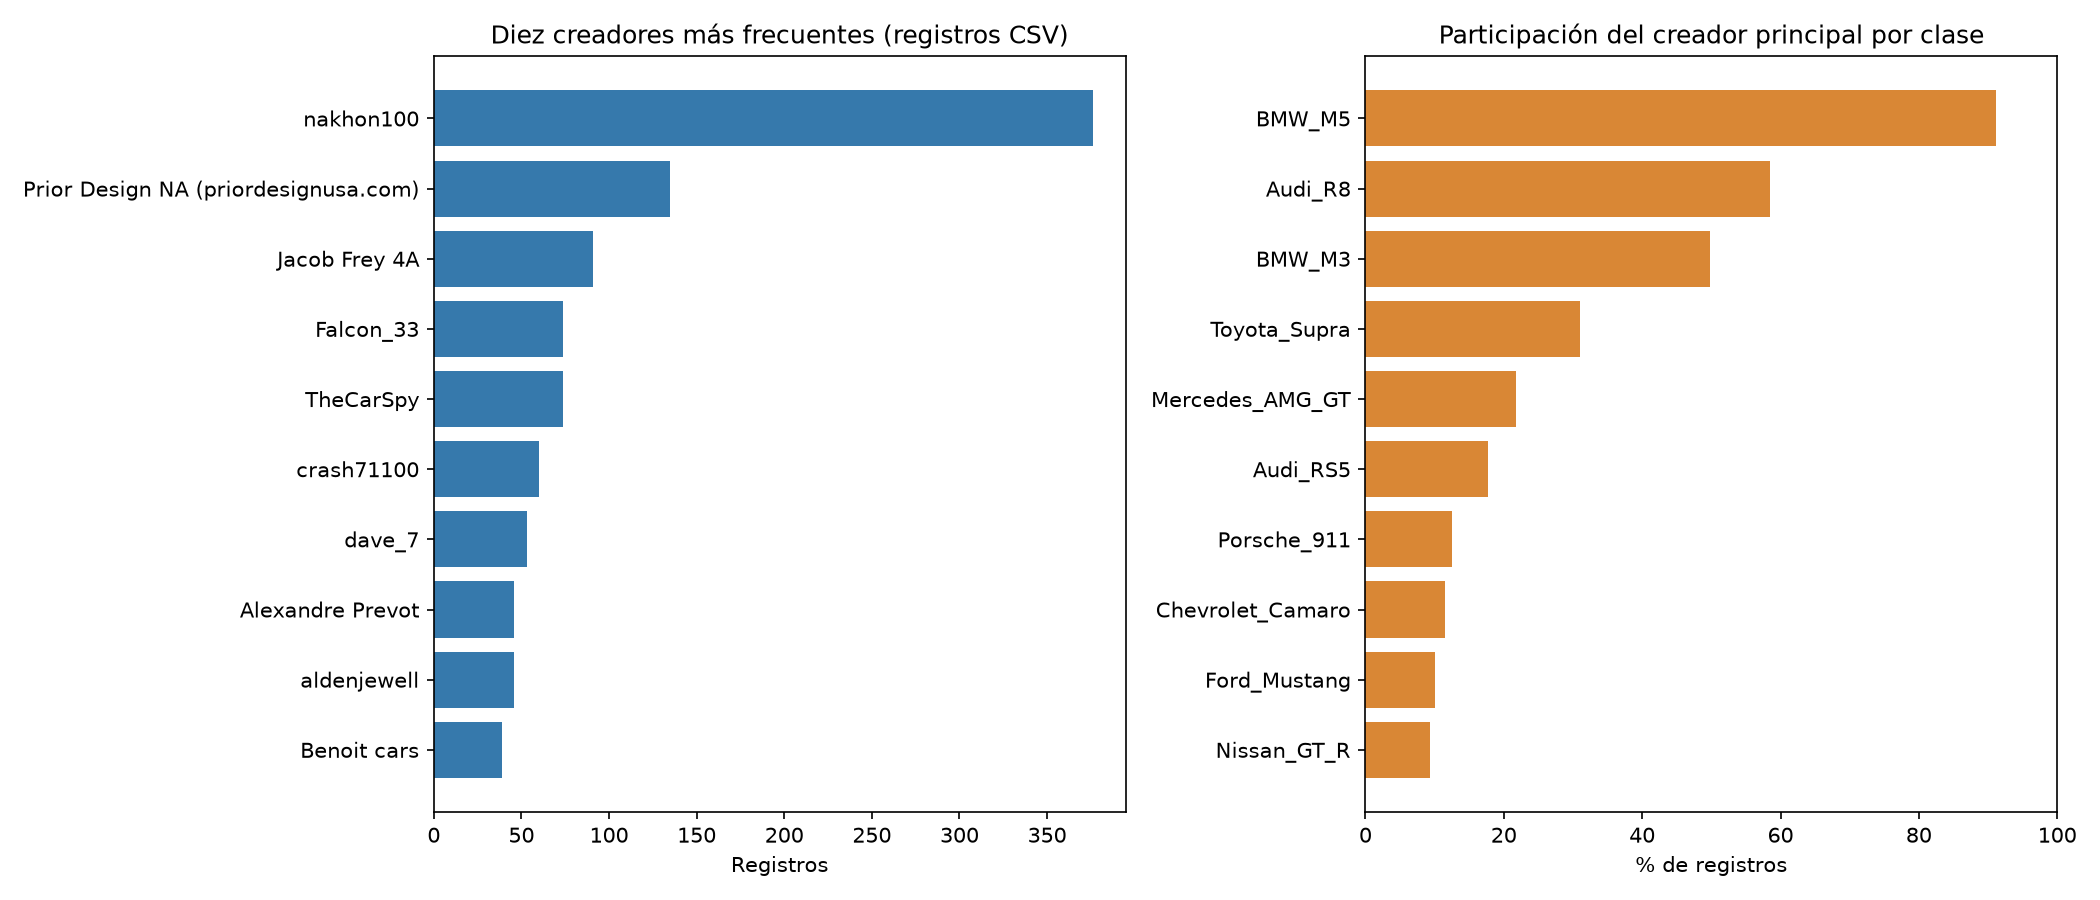
\includegraphics[width=0.92\textwidth,height=0.26\textheight,keepaspectratio]{eda/eda_procedencia_creadores.png}
\caption{Creadores más frecuentes y participación del principal creador en cada clase original. La concentración es particularmente alta en BMW M5. Fuente: análisis del campo de creador en los metadatos.}
\label{fig:autores}
\end{figure*}

Esto es importante porque si un autor utiliza escenarios, encuadres o marcas de agua similares, la red podría asociarlos con una clase. Esta posibilidad limita la interpretación de una partición aleatoria por imagen, ya que muchas fotografías no necesariamente representan una diversidad equivalente de vehículos o condiciones de captura. El aprendizaje de estos atajos permanece como una hipótesis.

\FloatBarrier
\section{Limpieza, transformación y conjuntos de datos}

\subsection{Duplicados y conflictos de etiquetas}

Se comparan dos formas de identidad exacta, SHA-256 de los archivos e identidad de los píxeles RGB después de corregir la orientación, la primera identifica archivos iguales, mientras que la segunda permite reconocer contenido decodificado idéntico. En este dataset, ambos criterios señalan los mismos nueve pares, es decir, 18 rutas únicas. 

Seis pares tienen etiquetas distintas pero representan la misma imagen o muy similar: uno entre BMW M3 y BMW M5, y cinco entre Chevrolet Camaro y Ford Mustang. La Figura~\ref{fig:duplicados} presenta algunos ejemplos. En escenas con varios vehículos puede haber más de una categoría visible, pero asignar etiquetas diferentes a la misma imagen genera una supervisión ambigua para una tarea de una sola salida. Se excluyen ambos miembros de esos seis pares, sin intentar averiguar cuál etiqueta es correcta. De los tres pares restantes se conserva una copia por orden alfabético de ruta.

% Detalle de los cuatro primeros pares del mosaico, sin modificar el PNG.
\begin{figure}[!htbp]
\centering
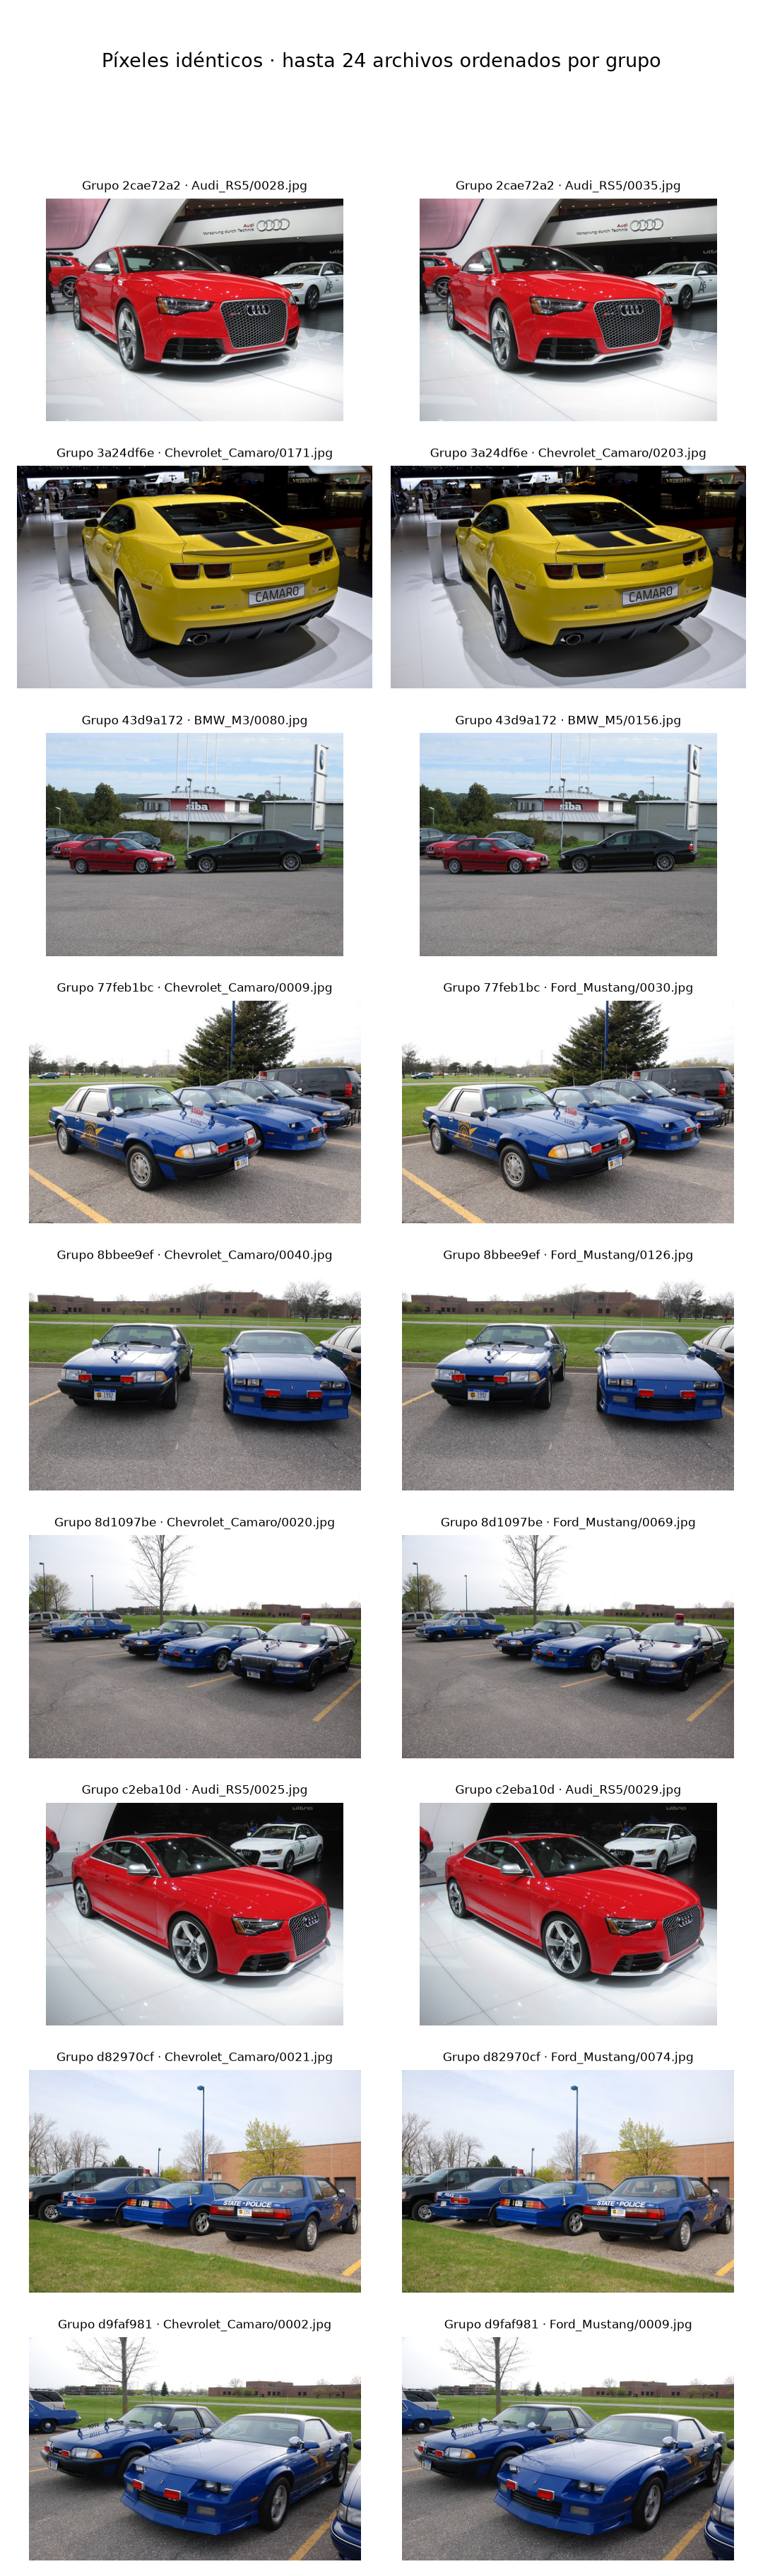
\includegraphics[trim=0 910bp 0 35bp,clip,width=\columnwidth,height=0.60\textheight,keepaspectratio]{eda/eda_duplicados_exactos.png}
\caption{Detalle de los primeros cuatro pares del mosaico de duplicados exactos, dos con la misma clase y dos con etiquetas distintas.}
\label{fig:duplicados}
\end{figure}

\begin{figure*}[!t]
\centering
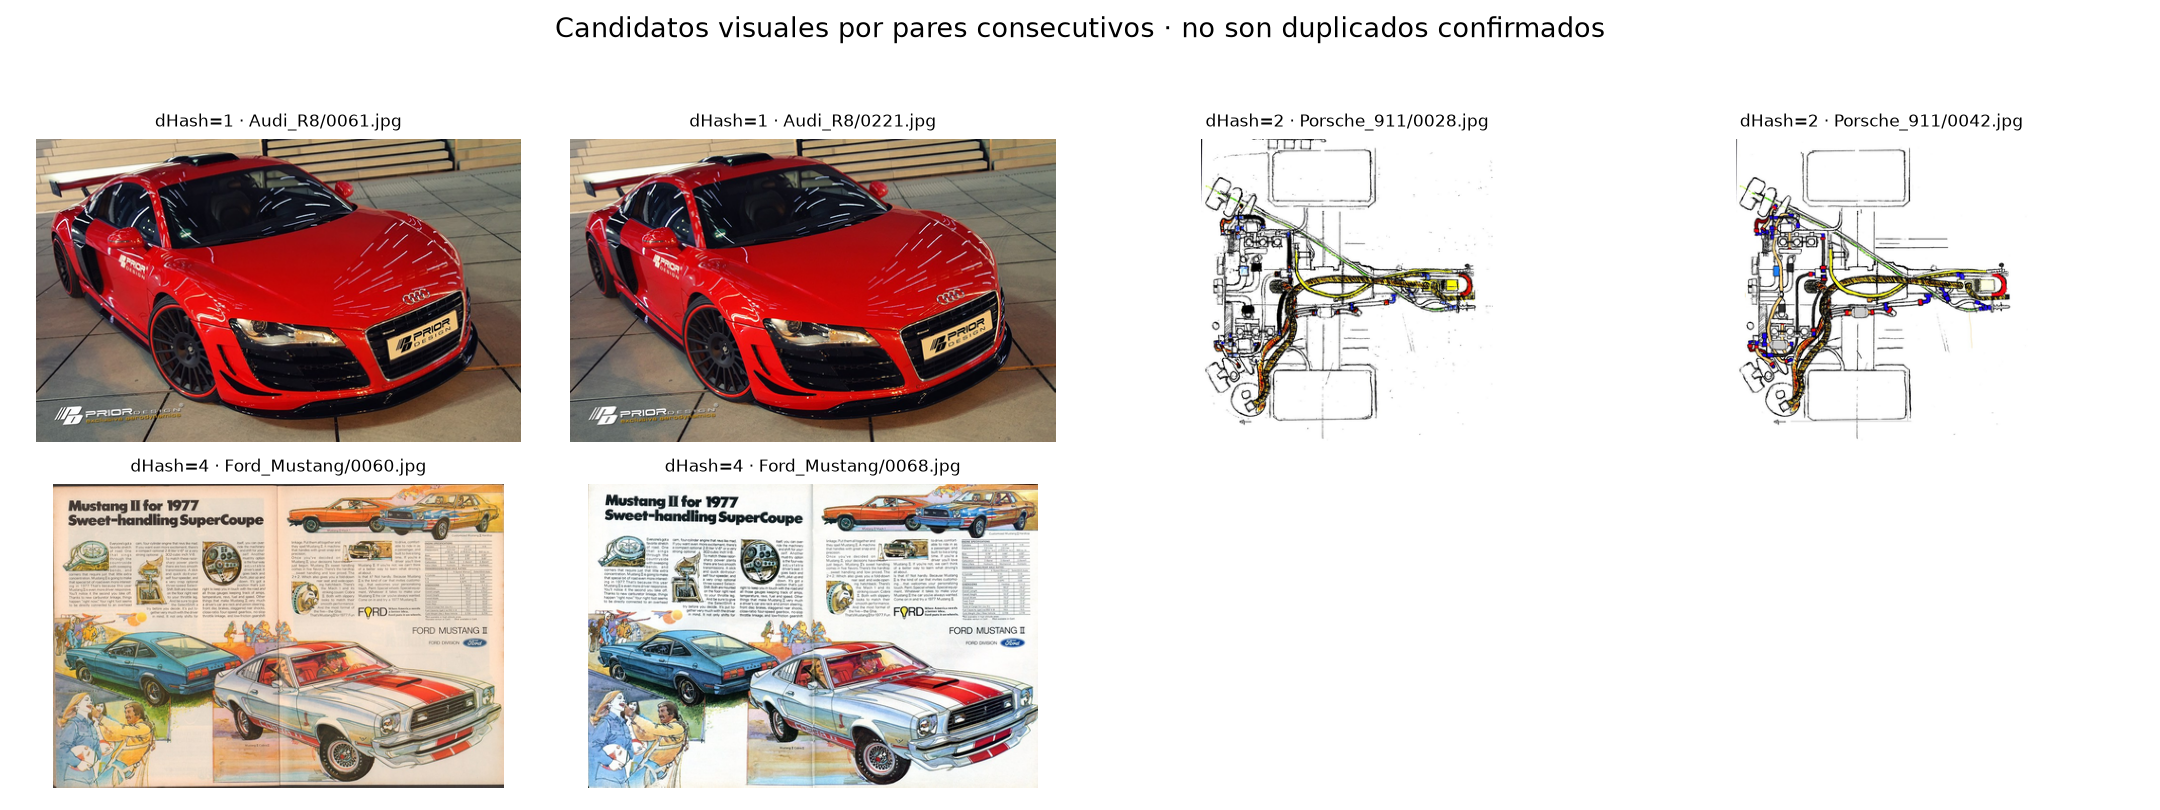
\includegraphics[width=0.92\textwidth]{eda/eda_similares_misma_clase.png}
\caption{Los tres pares candidatos por similitud dHash, ordenados por distancia.}
\label{fig:similares}
\end{figure*}

Además, se comparan huellas perceptuales dHash de 64 bits con distancia de Hamming de hasta cinco. Este criterio identifica tres pares candidatos dentro de Audi R8, Porsche 911 y Ford Mustang, con la Figura~\ref{fig:similares} muestra que el contenido incluye tanto fotografías como esquemas y material publicitario.

Una distancia pequeña en dHash indica una estructura visual parecida, sin confirmar duplicación. La exclusión automática puede reducir repetición o retirar variaciones útiles.

\begin{table}[!htbp]
\caption{Balance de imágenes durante la limpieza}
\label{tab:limpieza}
\centering
\small
\begin{tabular}{lr}
\toprule
Concepto & Imágenes \\
\midrule
Entrada original & 2,084 \\
Retiradas por conflicto de etiquetas & 12 \\
Copias exactas adicionales retiradas & 3 \\
Candidatos similares retirados & 3 \\
\midrule
Dataset resultante & 2,066 \\
\bottomrule
\end{tabular}
\par\smallskip
\begin{minipage}{\columnwidth}\scriptsize
Nota. Las exclusiones son mutuamente excluyentes. El balance se obtiene de los reportes de duplicados y candidatos y de la selección implementada: $2{,}084-12-3-3=2{,}066$.
\end{minipage}
\end{table}

La Tabla~\ref{tab:limpieza} resume la reducción de imagenes, es importante mencionar que la limpieza ocurre antes de la división de conjuntos para evitar que las copias detectadas terminen en conjuntos distintos, lo que reduce una fuga de información.

\vspace{2cm}

\subsection{Transformación de las imágenes}

Primero se aplica la orientación EXIF y se convierte la imagen a RGB, de manera que la entrada tenga tres canales. Después se ajusta dentro de un cuadrado de $224\times224$, manteniendo la relación de aspecto y sin recortar el contenido. Se aplica un filtro gaussiano de radio 1 a la imagen ajustada y se completa el espacio restante con relleno negro centrado. El resultado se guarda como JPEG con calidad 95.

El ajuste proporcional evita deformar elementos como faros, parrillas y también evita recortes automáticos que podrían eliminar el carro, aunque mantiene fondos y objetos ajenos a la clase. El relleno introduce pixeles negros cuyo tamaño depende de la proporción original. Este tamaño elegido reduce el costo de trabajar con los originales, a cambio de perder pequeños detalles.

El suavizado gaussiano puede disminuir variaciones de alta frecuencia, pero también difuminar emblemas o bordes discriminantes.

Al cargar la imagen procesada se convierten sus intensidades a punto flotante de 32 bits y se normalizan mediante
\begin{equation}
\widetilde{x}_{i,j,c}=\frac{x_{i,j,c}}{255},\qquad 0\leq\widetilde{x}_{i,j,c}\leq1,
\label{eq:normalizacion}
\end{equation}
donde $x_{i,j,c}$ es la intensidad del píxel en fila $i$, columna $j$ y canal $c$. Esta transformación unifica la escala de entrada, lo que resulta en que la forma final de cada ejemplo es $224\times224\times3$.

\subsection{Partición y carga para el aprendizaje}

El conjunto procesado se divide en 70\% para entrenamiento, 15\% para validación y 15\% para prueba, mediante dos separaciones estratificadas con semilla 42. La primera reserva 30\% y la segunda divide esa reserva en partes iguales. El redondeo produce 1,446 imágenes de entrenamiento y 310 en cada conjunto restante.

El conjunto de entrenamiento se utiliza para actualizar los pesos, validación permite observar el comportamiento fuera de esos ejemplos y elegir cuándo detenerse y prueba evalúa el modelo resultante. La estratificación mantiene aproximadamente las proporciones de clase y evita que las categorías menos frecuentes desaparezcan de algún conjunto.

Las imágenes se cargan por lotes de hasta 32 y las diez etiquetas se representan con enteros de 0 a 9 en orden alfabético, que representan únicamente la salida correspondiente.

\FloatBarrier
\section{Conceptos y decisiones del modelo}

\subsection{Convoluciones y aprendizaje de características}

La CNN busca aprender características útiles para separar las diez clases sin definir manualmente una variable para cada faro, rueda o parrilla. 

Los pesos  permiten buscar un patrón en distintas regiones con un mismo filtro, al aumentar los filtros se pueden representar más patrones y las capas posteriores combinan sus respuestas. Esto permite construir representaciones más complejas.

Las convoluciones implementadas tienen paso uno y relleno \textit{same}, por lo que conservan las dimensiones espaciales de su entrada antes del pooling. Su cantidad de parámetros se calcula como
\begin{equation}
P_{\mathrm{conv}}=(3\cdot3\cdot C+1)F,
\label{eq:parametros}
\end{equation}
con $F$ filtros y un sesgo por filtro. La Tabla~\ref{tab:arquitectura} presenta el recorrido completo. Por ejemplo, la primera convolución tiene $(9\cdot3+1)16=448$ parámetros.

\begin{table}[!htbp]
\caption{Arquitectura de la CNN y parámetros entrenables}
\label{tab:arquitectura}
\centering
\scriptsize
\setlength{\tabcolsep}{3pt}
\begin{tabular}{llr}
\toprule
Operación & Salida & Parámetros \\
\midrule
Entrada RGB & $224\times224\times3$ & 0 \\
Conv. $3\times3$, 16, ReLU & $224\times224\times16$ & 448 \\
Max pooling $4\times4$ & $56\times56\times16$ & 0 \\
Conv. $3\times3$, 32, ReLU & $56\times56\times32$ & 4,640 \\
Max pooling $4\times4$ & $14\times14\times32$ & 0 \\
Conv. $3\times3$, 64, ReLU & $14\times14\times64$ & 18,496 \\
Max pooling $4\times4$ & $4\times4\times64$ & 0 \\
Conv. $3\times3$, 128, ReLU & $4\times4\times128$ & 73,856 \\
Max pooling $4\times4$ & $1\times1\times128$ & 0 \\
Aplanado & 128 & 0 \\
Densa, ReLU & 128 & 16,512 \\
Densa, softmax & 10 & 1,290 \\
\midrule
Total & & 115,242 \\
\bottomrule
\end{tabular}
\end{table}

\subsection{Función ReLU}

Después de cada convolución y en la capa densa intermedia se utiliza la unidad lineal rectificada:
\begin{equation}
\operatorname{ReLU}(z)=\max(0,z).
\label{eq:relu}
\end{equation}
ReLU introduce una transformación no lineal que conserva los valores positivos y convierte los negativos en cero. En esta red, ReLU permite combinar las respuestas de los filtros de una forma que depende de los patrones presentes en cada imagen.

\subsection{Max pooling y reducción espacial}

Después de cada convolución se aplica max pooling con ventana y paso definidas. Esta técnica permite conservar la respuesta máxima de cada región, reduciendo las posiciones que procesan las capas siguientes sin añadir parámetros entrenables. El pooling conserva respuestas fuertes, aunque descarta la ubicación exacta de otras activaciones.

Con relleno \textit{same}, las dimensiones de salida se redondean hacia arriba al dividir por cuatro. Por ello, la secuencia es $224\rightarrow56\rightarrow14\rightarrow4\rightarrow1$, de acuerdo con la definición de la operación \citep{kerasPooling}. 

Esta reducción mantiene pequeño el número de conexiones densas, pero podría descartar detalles o relaciones espaciales necesarios. Los resultados de arquitecturas ligeras en otros dominios \citep{appasami2025} no prueban que esta reducción sea óptima para carros. 

\subsection{Capas densas, softmax y función de pérdida}

El aplanado convierte la representación $1\times1\times128$ en 128 valores sin aprender nuevos pesos. La capa densa siguiente combina esos valores en 128 unidades ReLU. Finalmente, diez\textit{logits}, se transforman con softmax:
\begin{equation}
\widehat{p}_{i,k}=\frac{\exp(z_{i,k})}{\sum_{j=1}^{K}\exp(z_{i,j})},
\qquad K=10.
\label{eq:softmax}
\end{equation}
Aquí $z_{i,k}$ es la puntuación de la clase $k$ para la imagen $i$, las salidas de todas las clases son positivas y deben sumar uno (100\%), para seleccionar la predicción se usa la clase con mayor valor. 

Se minimiza la entropía cruzada categórica con etiquetas enteras:
\begin{equation}
\mathcal{L}=-\frac{1}{N}\sum_{i=1}^{N}\log\widehat{p}_{i,y_i},
\label{eq:perdida}
\end{equation}
donde $y_i$ es la clase correcta y $N$ el número de ejemplos considerado. La denominación \textit{sparse} indica que la etiqueta se proporciona como un entero, sin exigir una representación one-hot explícita.

La pérdida considera cuánta probabilidad se asigna a la clase correcta, no únicamente si esta obtiene el máximo, por lo que, un error muy grande puede aumentar mucho la pérdida aunque el número total de aciertos apenas cambie. Esta distinción permite interpretar las curvas cuando la exactitud se mantiene estable y la pérdida de validación aumenta.

\FloatBarrier
\section{Entrenamiento y evaluación de la CNN v1}

\subsection{Configuración e hiperparámetros}

La red se entrena desde cero en CPU con TensorFlow/Keras, en cada lote se calcula la pérdida y se propaga su gradiente desde la salida hacia los parámetros de las capas anteriores mediante la regla de la cadena. Este proceso, conocido como retropropagación, determina cómo modificar los pesos para reducir el error observado.

Se utiliza Adam con tasa de aprendizaje 0.001, ya que, dam mantiene estimaciones de primer y segundo momento del gradiente para adaptar las actualizaciones de cada parámetro \citep{kingma2015} y la tasa controla la escala de esas actualizaciones, pero su valor no representa una garantía de convergencia ni de generalización. Por otro lado, Los lotes de 32 permiten actualizar la red con grupos de ejemplos. Con 1,446 imágenes se requieren 46 lotes por época.

\begin{table}[!htbp]
\caption{Configuración del entrenamiento analizado}
\label{tab:entrenamiento}
\centering
\small
\begin{tabularx}{\columnwidth}{lX}
\toprule
Elemento & Configuración \\
\midrule
Entrada & $224\times224\times3$, valores entre 0 y 1 \\
Optimizador & Adam, tasa de aprendizaje 0.001 \\
Pérdida & Entropía cruzada categórica con etiquetas enteras \\
Lote & Hasta 32 imágenes \\
Máximo de épocas & 30 \\
Detención temprana & Mínima pérdida de validación; paciencia 5 \\
Pesos finales & Restauración de los mejores de validación \\
Semilla & 42 para partición, inicialización y mezcla \\
\bottomrule
\end{tabularx}
\end{table}

\subsection{Detención temprana y selección de pesos}

El \textit{early stopping} monitorea la pérdida de validación y detiene el entrenamiento después de cinco épocas consecutivas sin disminuirla. Al finalizar, restaura los pesos asociados con el menor valor registrado \citep{kerasEarly}. De esta forma se evita conservar automáticamente la última época, que puede ajustarse mejor al entrenamiento y peor a ejemplos reservados.

Las gráficas disponibles contienen 17 épocas, donde el mínimo de validación se aprecia alrededor de la época 12 y después la pérdida aumenta durante las cinco siguientes. La detención temprana limita la degradación posterior, pero no corrige por sí misma la falta de diversidad, las etiquetas ambiguas ni la información descartada durante el procesamiento.

En las curvas, entrenamiento es el promedio de los lotes mientras los pesos cambian durante la época. Validación y prueba se evalúan al terminarla. Las métricas finales se vuelven a calcular para los tres conjuntos con los pesos restaurados y sin mezclar el orden de evaluación.

\subsection{Métricas utilizadas}

La exactitud mide la proporción de imágenes cuya predicción coincide con la etiqueta:
\begin{equation}
\operatorname{Accuracy}=\frac{1}{N}\sum_{i=1}^{N}\mathbf{1}(\widehat{y}_i=y_i).
\label{eq:accuracy}
\end{equation}
El indicador $\mathbf{1}$ vale uno cuando hay coincidencia y cero en caso contrario, es decir, para cada clase $k$, se consideran positivos sus ejemplos y negativos los de las otras nueve. Los verdaderos positivos $TP_k$ son sus aciertos, los falsos positivos $FP_k$ son imágenes ajenas asignadas a ella, y los falsos negativos $FN_k$ son sus imágenes asignadas a otra categoría. Entonces,
\begin{align}
\operatorname{Precision}_k&=\frac{TP_k}{TP_k+FP_k},\label{eq:precision}\\
\operatorname{Recall}_k&=\frac{TP_k}{TP_k+FN_k},\label{eq:recall}\\
F1_k&=\frac{2\operatorname{Precision}_k\operatorname{Recall}_k}
{\operatorname{Precision}_k+\operatorname{Recall}_k}.\label{eq:f1}
\end{align}

La precisión responde qué proporción de las predicciones de una clase es correcta. Recall indica qué proporción de sus ejemplos reales se recupera. F1 combina ambas mediante una media armónica y penaliza que alguna sea baja.

Para una métrica por clase $m_k$, el promedio macro se define como
\begin{equation}
m_{\mathrm{macro}}=\frac{1}{K}\sum_{k=1}^{K}m_k.
\label{eq:macro}
\end{equation}
En particular, el F1 macro promedia los diez valores de $F1_k$, así se conserva la importancia de Audi RS5 y Mercedes AMG GT aunque tengan menos ejemplos.

\FloatBarrier
\section{Resultados obtenidos}

\subsection{Desempeño global con los pesos restaurados}

La Tabla~\ref{tab:metricas} transcribe las etiquetas numéricas del reporte final mostrado en la Figura~\ref{fig:metricas}, que representan valores redondeados a tres decimales.

\begin{table}[!htbp]
\caption{Métricas finales con los mejores pesos de validación}
\label{tab:metricas}
\centering
\scriptsize
\setlength{\tabcolsep}{3pt}
\begin{tabular}{lrrrr}
\toprule
Conjunto & Accuracy & Prec. macro & Recall macro & F1 macro \\
\midrule
Train & 0.464 & 0.486 & 0.454 & 0.423 \\
Validación & 0.294 & 0.290 & 0.283 & 0.245 \\
Prueba & 0.310 & 0.304 & 0.297 & 0.273 \\
\bottomrule
\end{tabular}
\par\smallskip
\end{table}

\begin{figure}[!htbp]
\centering
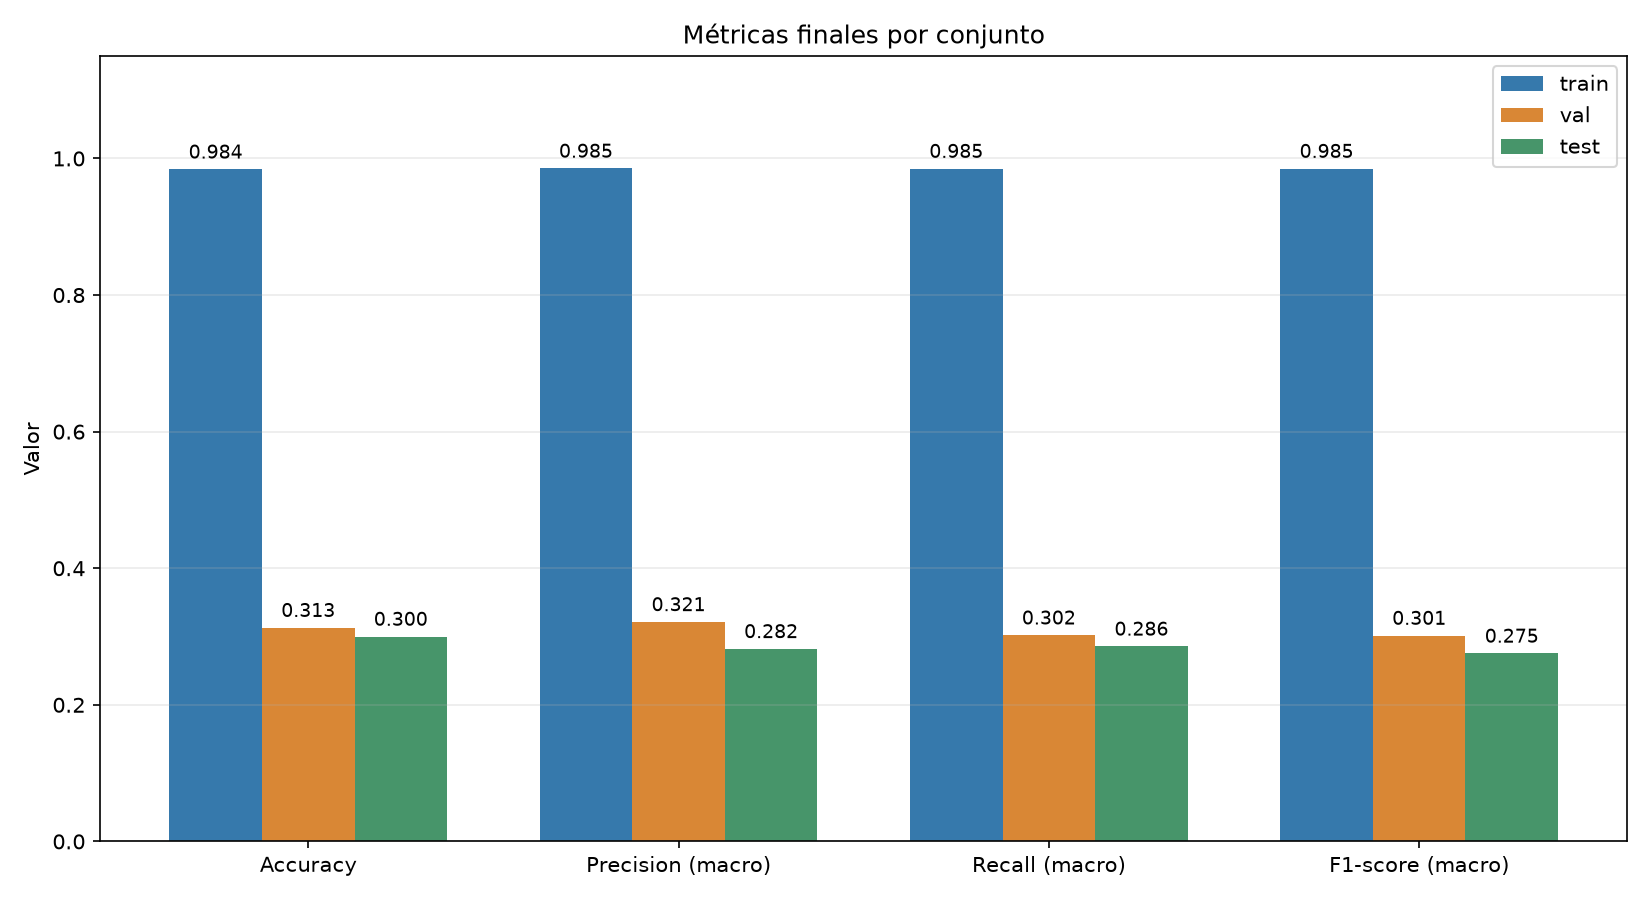
\includegraphics[width=\columnwidth]{cnn_v1/cnn_v1_metrics.png}
\caption{Reporte de exactitud, precisión macro, recall macro y F1 macro, con los mejores resultados tras aplicar early stopping.}
\label{fig:metricas}
\end{figure}

La exactitud de prueba indica que se reconoce aproximadamente 31\% de los ejemplos reservados, mientras que cerca de 69\% se asigna a otra clase. En la matriz se cuentan 96 aciertos de 310. 

El F1 macro de prueba, 0.273, muestra que el equilibrio entre precisión y recuperación es limitado al dar el mismo peso a todas las categorías.

La diferencia aproximada entre exactitud final de entrenamiento y prueba es de 15.4 puntos porcentuales, y respecto de validación es de 17.0. El modelo aprovecha mejor los ejemplos usados para ajustar sus parámetros. Validación y prueba tienen resultados cercanos, aunque el valor algo mayor de prueba no demuestra una mejora,

\subsection{Curvas de aprendizaje y sobreajuste}

\begin{figure*}[!t]
\centering
\begin{minipage}{0.49\textwidth}
\centering
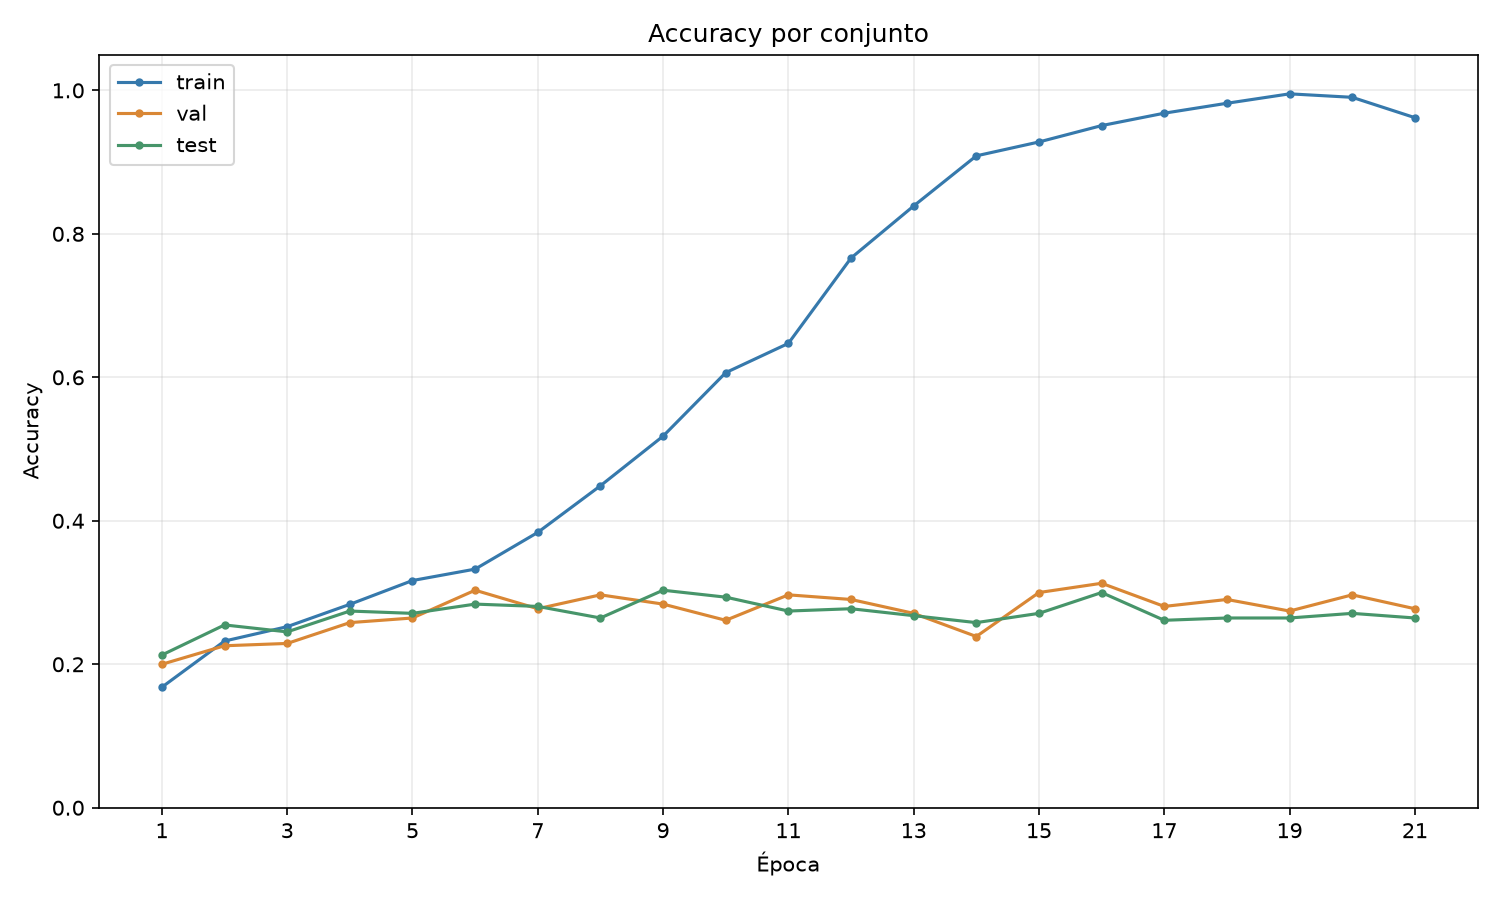
\includegraphics[width=\linewidth]{cnn_v1/cnn_v1_accuracy.png}
\end{minipage}\hfill
\begin{minipage}{0.49\textwidth}
\centering
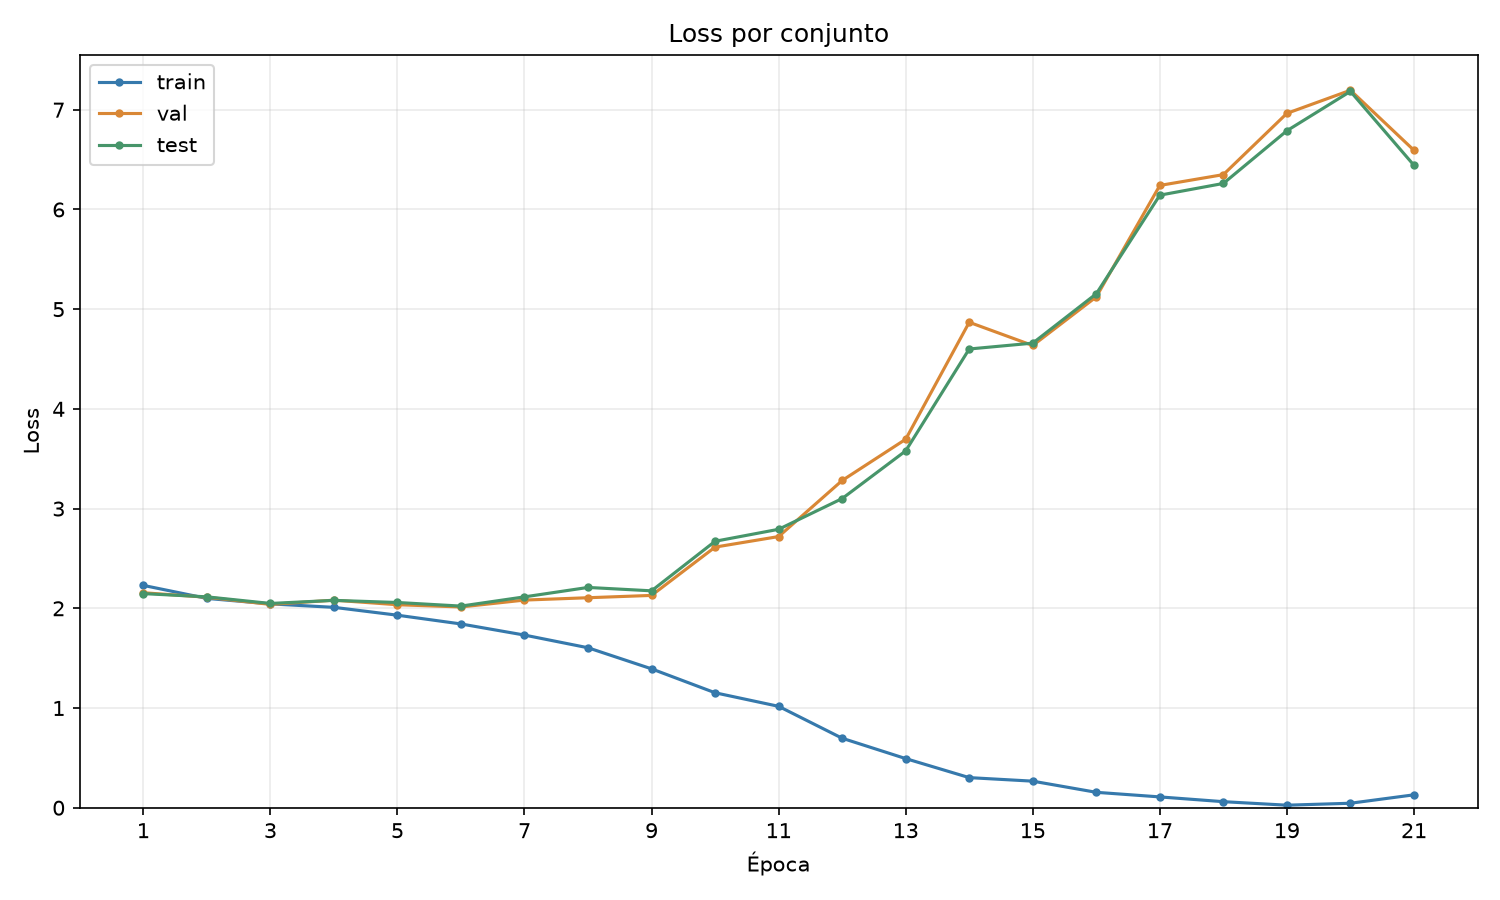
\includegraphics[width=\linewidth]{cnn_v1/cnn_v1_loss.png}
\end{minipage}
\caption{Exactitud y pérdida durante las 17 épocas registradas.}
\label{fig:curvas}
\end{figure*}

La Figura~\ref{fig:curvas} permite observar una separación progresiva. La exactitud de entrenamiento aumenta hasta aproximadamente 0.62 en la época 17; validación y prueba varian alrededor de 0.2 a 0.3. Al mismo tiempo, la pérdida de entrenamiento disminuye, mientras que las pérdidas de evaluación dejan de mejorar y aumentan al final.

Este patrón es evidencia de sobreajuste, donde reducir el error en los ejemplos de aprendizaje ya no produce una mejora comparable fuera de ellos.

También se observa por qué la pérdida aporta información adicional a la exactitud, ya que la red puede conservar un número parecido de aciertos y volverse más confiada en sus errores. En este caso, la entropía cruzada aumenta aunque apenas cambie la clase con mayor probabilidad, por eso se utiliza la pérdida de validación para detenerse y no únicamente la exactitud.

\subsection{Matriz de confusión y diferencias entre clases}

\begin{figure*}[!t]
\centering
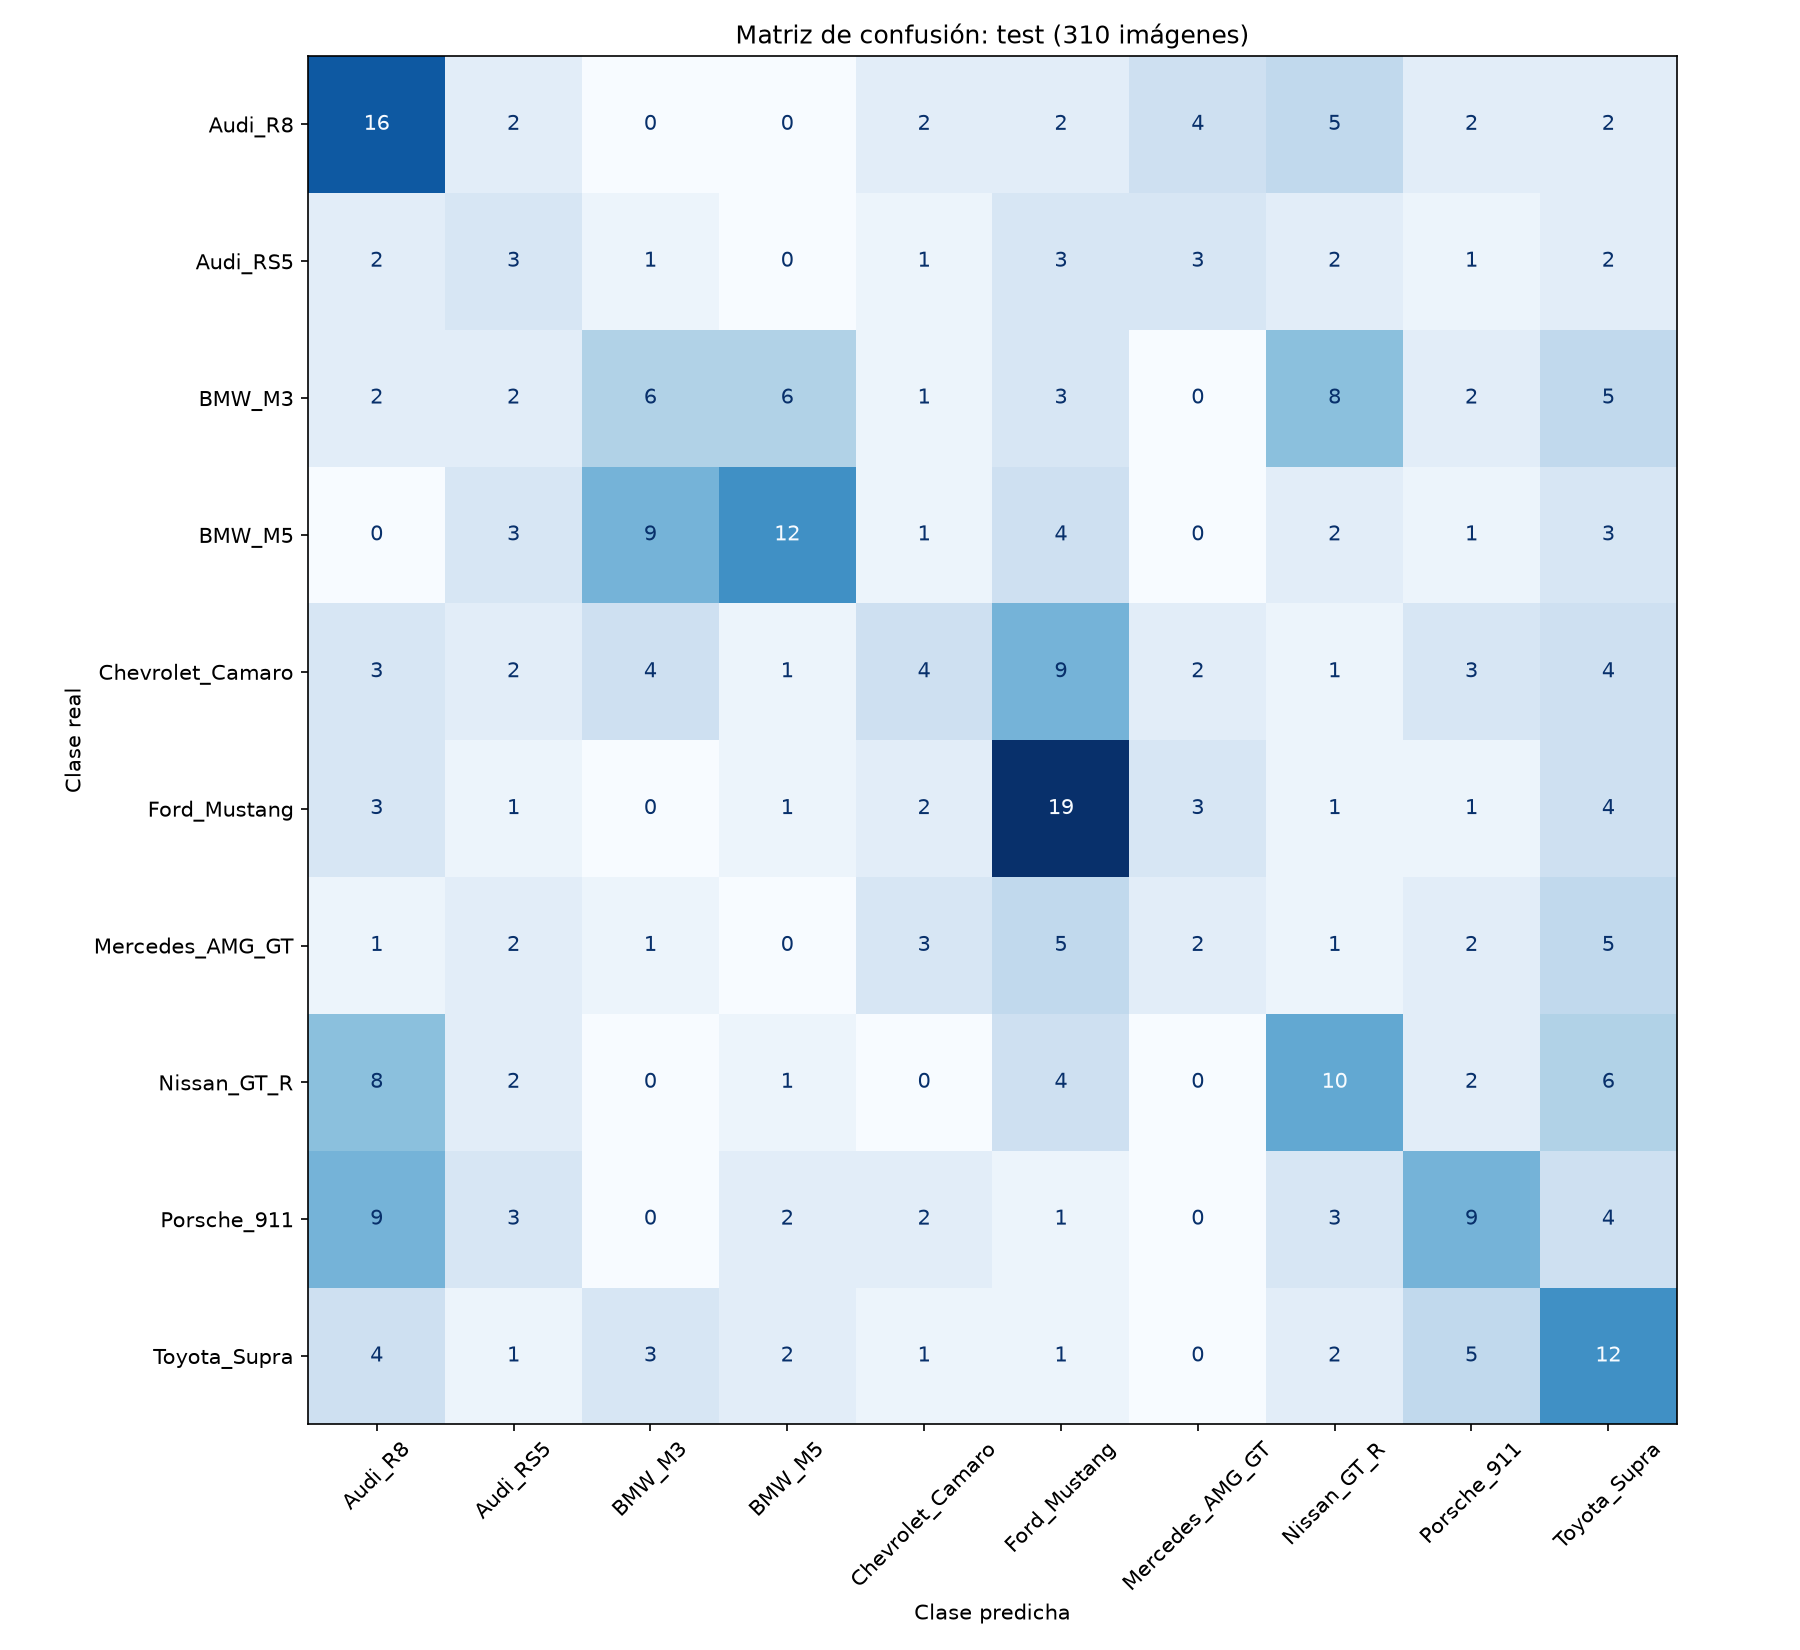
\includegraphics[width=0.76\textwidth,height=0.70\textheight,keepaspectratio]{cnn_v1/cnn_v1_confusion_test.png}
\caption{Matriz de confusión final de prueba, con 310 imágenes. Las filas son clases reales y las columnas clases predichas.}
\label{fig:confusion}
\end{figure*}

La Figura~\ref{fig:confusion} presenta cantidades absolutas, cada fila corresponde a una clase real y cada columna predicha, la diagonal contiene los aciertos. La Tabla~\ref{tab:recallclases} divide los aciertos por el total real de cada fila.

\begin{table}[!htbp]
\caption{Aciertos y recuperación por clase en prueba}
\label{tab:recallclases}
\centering
\small
\begin{tabular}{lrrr}
\toprule
Clase & Aciertos & Soporte & Recall (\%) \\
\midrule
Audi R8 & 15 & 35 & 42.9 \\
Audi RS5 & 1 & 18 & 5.6 \\
BMW M3 & 1 & 35 & 2.9 \\
BMW M5 & 26 & 35 & 74.3 \\
Chevrolet Camaro & 13 & 33 & 39.4 \\
Ford Mustang & 11 & 35 & 31.4 \\
Mercedes AMG GT & 8 & 22 & 36.4 \\
Nissan GT-R & 7 & 33 & 21.2 \\
Porsche 911 & 9 & 33 & 27.3 \\
Toyota Supra & 5 & 31 & 16.1 \\
\midrule
Total & 96 & 310 & --- \\
\bottomrule
\end{tabular}
\par\smallskip
\begin{minipage}{\columnwidth}\scriptsize
Nota. Soporte es el número real de ejemplos de la clase. La exactitud global es $96/310$, el recall macro promedia las diez tasas.
\end{minipage}
\end{table}

BMW M5 alcanza 26 aciertos de 35, mientras BMW M3 obtiene uno de 35, además, 16 imágenes de BMW M3 se predicen como BMW M5. Esta confusión es asimétrica porque solo una imagen de BMW M5 se asigna a BMW M3. 

Audi RS5 también tiene una recuperación baja, debido a que únicamente uno de sus 18 ejemplos se identifica correctamente, una posible causa es su menor cantidad de entrenamiento, pero no explica por sí sola el resultado, ya que BMW M3 tiene muchos más ejemplos y presenta una recuperación todavía menor.

Otros resultados son que diez imágenes de Nissan GT-R y diez de Porsche 911 se asignan a Audi R8, a su vez, ocho Audi R8 y ocho Ford Mustang se predicen como Mercedes AMG GT. Estas cantidades muestran que el error no está restringido a parejas de modelos cercanos. La revisión de ejemplos concretos permitiría estudiar si predominan encuadres parciales, fondos compartidos o características del vehículo.

BMW M5 recupera buena parte de sus ejemplos, pero también recibe errores de otras filas y su recall alto no implica que todas sus predicciones sean correctas.


\section{Conclusiones}
% por ahora nada

\begin{thebibliography}{8}

\bibitem[Appasami \& Savarimuthu(2025)]{appasami2025}
Appasami, G., \& Savarimuthu, N. (2025). A novel lightweight CNN design for MRI brain tumor image classification with performance-driven optimization. \textit{Discover Computing, 28}, Article 206. \url{https://doi.org/10.1007/s10791-025-09603-4}

\bibitem[Goodfellow et al.(2016)]{goodfellow2016}
Goodfellow, I., Bengio, Y., \& Courville, A. (2016). \textit{Deep learning}. MIT Press. \url{https://www.deeplearningbook.org/}

\bibitem[Keras(s.f.-a)]{kerasEarly}
Keras. (s.f.-a). \textit{EarlyStopping}. Recuperado el 26 de octubre de 2026, de \url{https://keras.io/api/callbacks/early_stopping/}

\bibitem[Keras(s.f.-b)]{kerasPooling}
Keras. (s.f.-b). \textit{MaxPooling2D layer}. Recuperado el 26 de octubre de 2026, de \url{https://keras.io/api/layers/pooling_layers/max_pooling2d/}

\bibitem[Khan et al.(2026)]{khan2026}
Khan, M. S., Siivola, E., \& Raitoharju, J. (2026). On class imbalance in machine learning-based taxa identification: A comparative analysis of mitigation strategies. \textit{Machine Learning with Applications, 24}, Article 100931. \url{https://doi.org/10.1016/j.mlwa.2026.100931}

\bibitem[Kingma \& Ba(2015)]{kingma2015}
Kingma, D. P., \& Ba, J. (2015). \textit{Adam: A method for stochastic optimization}. International Conference on Learning Representations. \url{https://arxiv.org/abs/1412.6980}

\bibitem[lightangle(s.f.)]{dataset}
lightangle. (s.f.). \textit{Car model image classification} [Conjunto de datos]. Kaggle. \url{https://www.kaggle.com/datasets/lightangle/car-model-image-classification}

\bibitem[Zhang et al.(2024)]{zhang2024}
Zhang, Y., Allen, T. T., \& Rodriguez Buno, R. (2024). Exploratory image data analysis for quality improvement hypothesis generation. \textit{Quality Engineering, 36}(4), 693--712. \url{https://doi.org/10.1080/08982112.2023.2285305}

\end{thebibliography}
\end{document}
